
\documentclass{article}
\usepackage[a4paper,margin=1in]{geometry}
\usepackage{tikz}
\usetikzlibrary{positioning, shapes.geometric}

\begin{document}

\section*{Frise chronologique du Musée de l'Air et de l'Espace}

\begin{center}
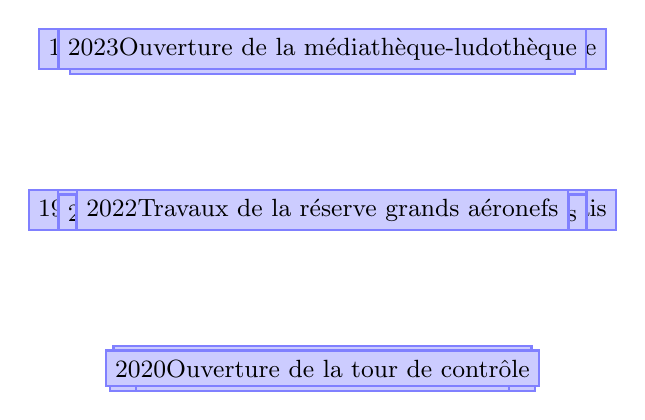
\begin{tikzpicture}[
    timeline/.style={rectangle, draw=blue!50, fill=blue!20, thick, minimum height=1.2em, text centered},
    every node/.style={font=\small},
    node distance=1.5cm and 2.5cm
  ]

% Dates et événements (alternance haut/bas)
\node[timeline] (d1918) {1918\\Création du Conservatoire de l’aéronautique};
\node[timeline, below=of d1918] (d1919) {1919\\Première exposition publique au Grand Palais};
\node[timeline, below=of d1919] (d1921) {1921\\Inauguration à Chalais-Meudon};
\node[timeline, above=of d1921] (d1936) {1936\\Transfert partiel à Paris, bd Victor};
\node[timeline, above=of d1936] (d1937) {1937\\Inauguration de l’aérogare du Bourget};
\node[timeline, below=of d1937] (d1940) {1940\\Bombardement et fermeture du musée};
\node[timeline, below=of d1940] (d1945) {1945\\Réouverture à Chalais-Meudon};
\node[timeline, above=of d1945] (d1951) {1951\\Création de l’AAMA};
\node[timeline, above=of d1951] (d1973) {1973\\Décision de transfert au Bourget};
\node[timeline, below=of d1973] (d1975) {1975\\Inauguration du premier hall au Bourget};
\node[timeline, below=of d1975] (d1981) {1981\\Fermeture de Chalais-Meudon};
\node[timeline, above=of d1981] (d1983) {1983\\Inauguration du hall de l’Espace};
\node[timeline, above=of d1983] (d1987) {1987\\Ouverture de la Grande Galerie};
\node[timeline, below=of d1987] (d1995) {1995\\Installation de la maquette Ariane 5};
\node[timeline, below=of d1995] (d1996) {1996\\Hangar pour Concorde 001};
\node[timeline, above=of d1996] (d2013) {2013\\Rénovation de la salle des Huit Colonnes};
\node[timeline, above=of d2013] (d2017) {2017\\Inauguration réserve Jean-Paul Béchat};
\node[timeline, below=of d2017] (d2019) {2019\\Centenaire et Grande Galerie rénovée};
\node[timeline, below=of d2019] (d2020) {2020\\Ouverture de la tour de contrôle};
\node[timeline, above=of d2020] (d2022) {2022\\Travaux de la réserve grands aéronefs};
\node[timeline, above=of d2022] (d2023) {2023\\Ouverture de la médiathèque-ludothèque};

\end{tikzpicture}
\end{center}

\end{document}
